% Created 2020-06-16 Di 10:05
% Intended LaTeX compiler: pdflatex
\documentclass[8pt]{beamer}
\usepackage[utf8]{inputenc}
\usepackage[T1]{fontenc}
\usepackage{graphicx}
\usepackage{grffile}
\usepackage{longtable}
\usepackage{wrapfig}
\usepackage{rotating}
\usepackage[normalem]{ulem}
\usepackage{amsmath}
\usepackage{textcomp}
\usepackage{amssymb}
\usepackage{capt-of}
\usepackage{hyperref}
\usetheme{default}
\author{Hanne, Talbot, Radzieda}
\date{2020-06-16}
\title{Digitale Signalverarbeitung in Python}
\hypersetup{
 pdfauthor={Hanne, Talbot, Radzieda},
 pdftitle={Digitale Signalverarbeitung in Python},
 pdfkeywords={},
 pdfsubject={},
 pdfcreator={Emacs 26.3 (Org mode 9.1.9)}, 
 pdflang={English}}
\begin{document}

\maketitle



\begin{frame}[label={sec:org7ee95bd}]{DSP mit Python - Inhalt}
\begin{itemize}
\item Vorstellung Bibliothek NumPy, SciPy, matplotlib
\item Vergleiche von Codebeispielen Python / Matlab
\item Geschwindigkeitsvergleiche
\item Hardwarebeschleunigung
\end{itemize}
\end{frame}


\begin{frame}[label={sec:org64f07e7}]{DSP mit Python - Numpy}
\begin{block}{NumPy}
\begin{itemize}
\item Bibliothek für mehrdimensionale Arrays, Matrizen und Vektoren
\item Entstanden 1995(als Numeric), 2006 als NumPy
\item Matlab 1984 (kommerziell)
\item NumPy / Matlab verwenden gleiche Libs
\end{itemize}
\end{block}
\end{frame}


\begin{frame}[label={sec:orgf83de88}]{DSP mit Python - Numpy}
\begin{columns}
\begin{column}{0.5\columnwidth}
\begin{block}{Erklärung}
\begin{itemize}
\item 2 zufällige Arrays/Listen werden erzeugt und jeweils zusammen addiert
\item für das Erzeugen, egal wie vielen Arrays, wird bei NumPy fast die gleiche Zeit benötigt
\end{itemize}
\end{block}
\end{column}

\begin{column}{0.5\columnwidth}
\begin{block}{Unterschied Array / Listen}
\begin{center}
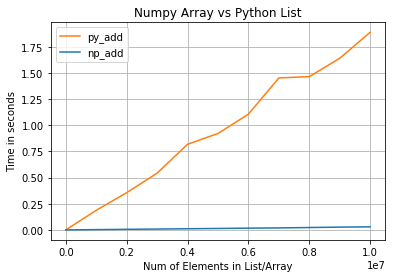
\includegraphics[width=.9\linewidth]{./image/vergleich_array.png}
\end{center}

\vspace{1mm}
Quelle Bild:
\url{https://miro.medium.com/max/792/1*rQoLViAcg2Hj8AD1EmONAg.png}
\end{block}
\end{column}
\end{columns}
\end{frame}


\begin{frame}[label={sec:org6404beb}]{DSP mit Python - Numpy}
\begin{block}{Python Listen}
\begin{itemize}
\item keine Angabe von Datentypen und Anzahl der Elemente
\item Daten von Listen sind im gesamten RAM verstreut und durch Zeiger referenziert
\item Standardmäßig 1-Dimensional (Bei n-Dimensionale Listen werden 1D Listen in einer 1D Liste gespeichert)
\item Elementweise Operationen auf Listen ist nicht möglich
\end{itemize}
\end{block}

\begin{block}{NumPy Array}
\begin{itemize}
\item Speichern einen definierten Datentyp
\item Anzahl der Elemente wird im voraus angegeben
\item Verbraucht weniger Speicher, da zusammenhängend im RAM gespeichert
\end{itemize}
\end{block}
\end{frame}


\begin{frame}[fragile,label={sec:orge388cf4}]{DSP mit Python - Numpy}
 \begin{block}{Python Liste}
\begin{verbatim}
>>> a = [1, 2, 3]
>>> b = [4, 5, 6]
>>> a + b
[1, 2, 3, 4, 5, 6]
\end{verbatim}
\end{block}
\begin{block}{np-Array}
\begin{verbatim}
>>> import numpy as np
>>> c = np.array([1, 2, 3])
>>> d = np.array([4, 5, 6])
>>> c + d
array([5, 7, 9])
\end{verbatim}
\end{block}
\end{frame}


\begin{frame}[fragile,label={sec:org262102d}]{DSP mit Python - Numpy}
 \begin{block}{Python Liste}
\begin{verbatim}
>>> a = [1, 2, 3]
>>> a * 3
[1, 2, 3, 1, 2, 3, 1, 2, 3]
\end{verbatim}
\end{block}
\begin{block}{np-Array}
\begin{verbatim}
>>> import numpy as np
>>> b = np.array([1, 2, 3])
>>> b * 3
array([3, 6, 9])
\end{verbatim}
\end{block}
\end{frame}


\begin{frame}[label={sec:orgdb8698f}]{DSP mit Python - SciPy und matplotlib}
\begin{block}{SciPy Funktionen}
\begin{itemize}
\item Gute Online-Dokumentation (\url{https://docs.scipy.org/doc/scipy/reference/})
\item cluster, fft, signal, stats uvm.
\item Basiert auf NumPy
\end{itemize}
\end{block}

\begin{block}{matplotlib}
\begin{itemize}
\item Eine Bibliothek zum Plotten von Grafen
\item sehr ähnliche Funktionen wie bei Matlab / Octave
\end{itemize}
\end{block}
\end{frame}


\begin{frame}[label={sec:org7b52c9d}]{DSP mit Python - matplotlib}
\begin{columns}
\begin{column}{0.5\columnwidth}
\begin{block}{Octave}
\begin{center}
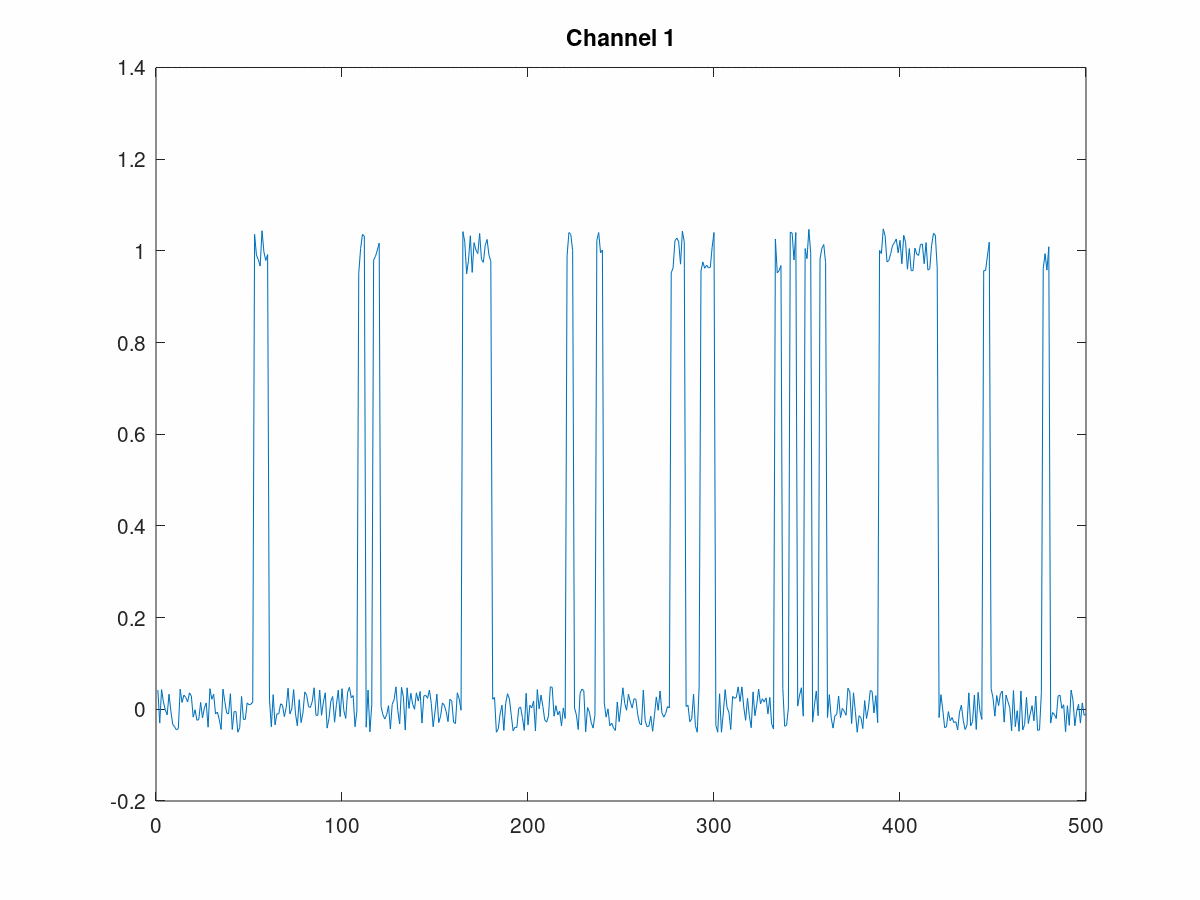
\includegraphics[width=.9\linewidth]{./image/vergleich_octave.png}
\end{center}
\end{block}
\end{column}

\begin{column}{0.5\columnwidth}
\begin{block}{matplotlib}
\begin{center}
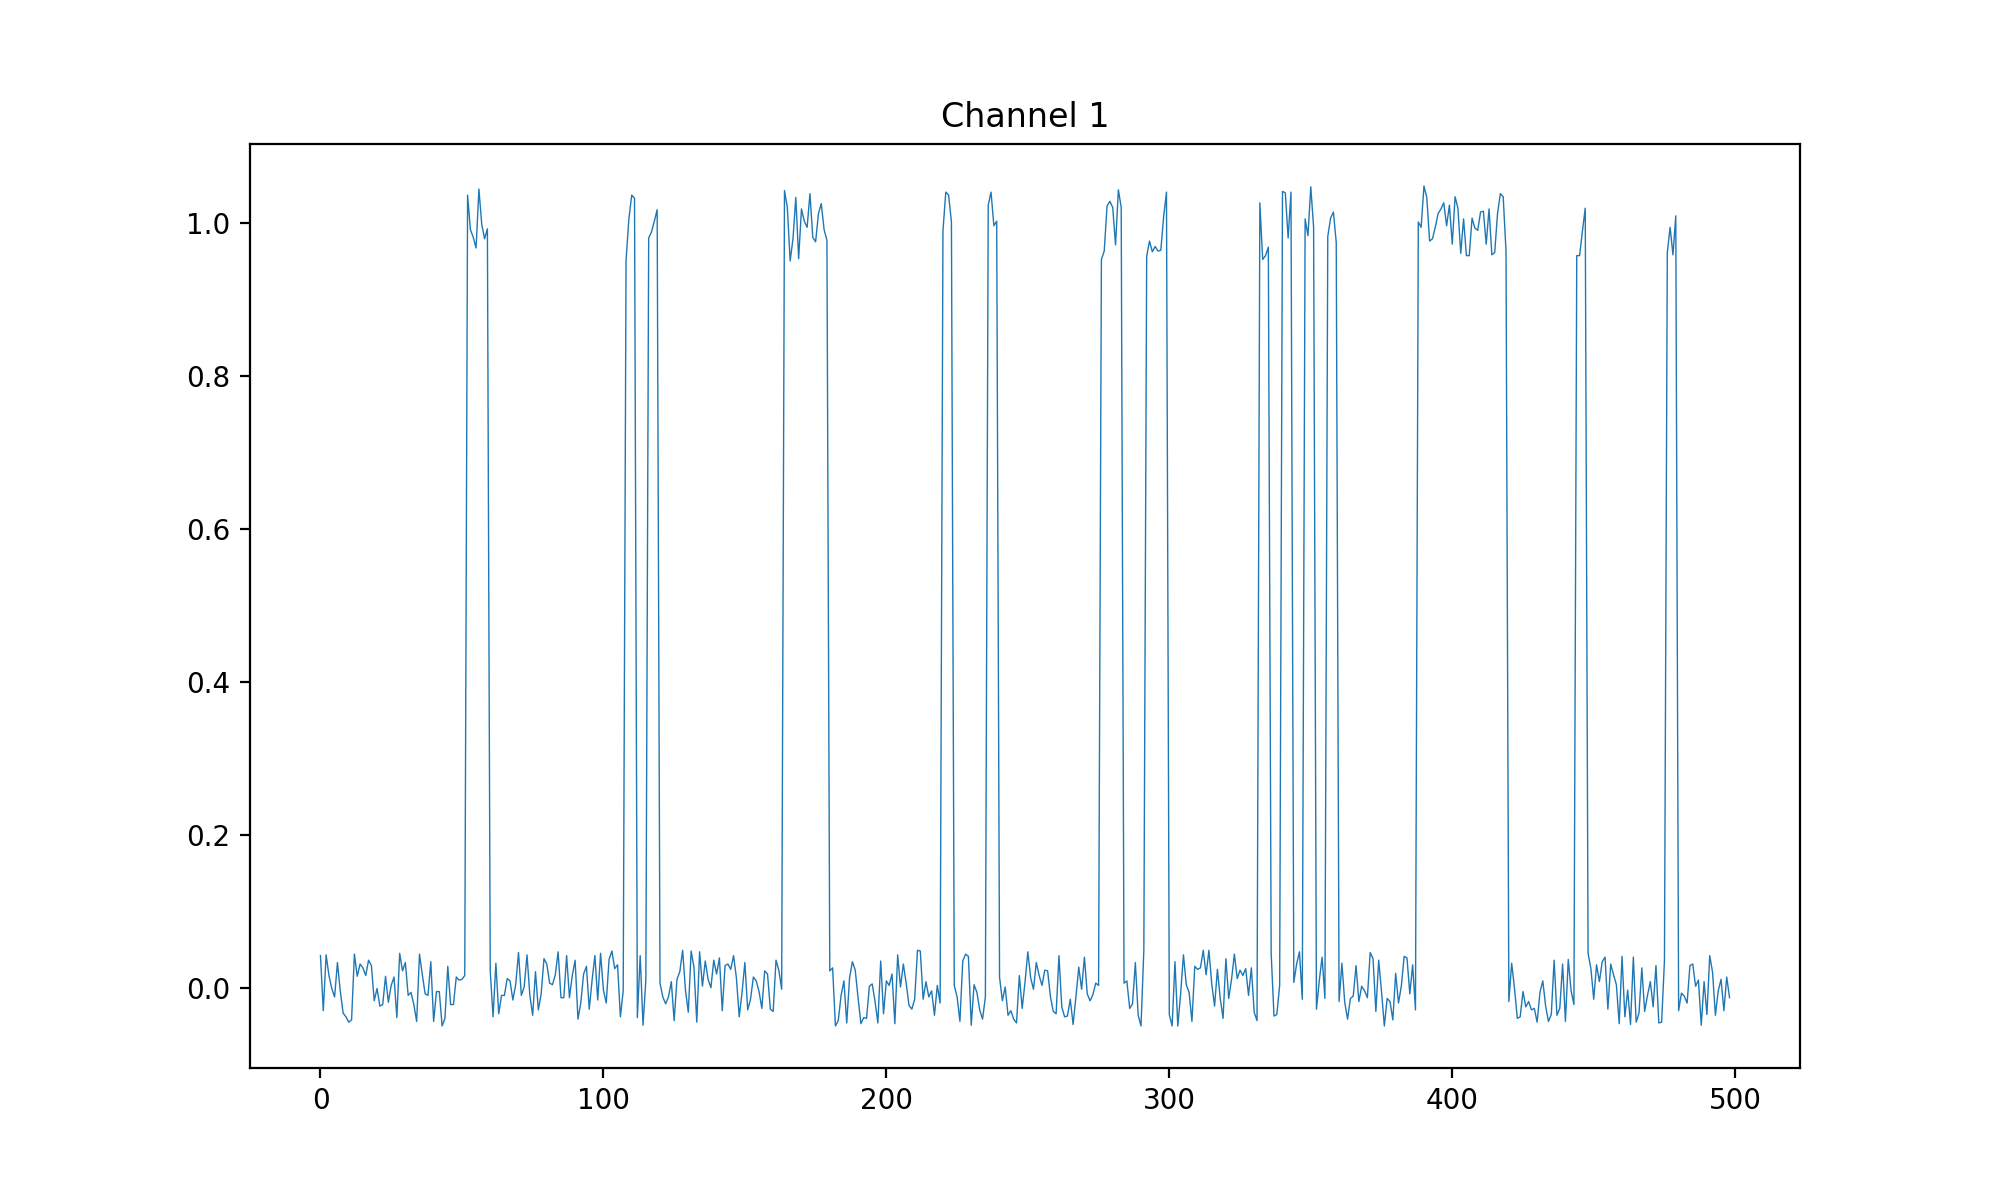
\includegraphics[width=.9\linewidth]{./image/Vergleich_python.png}
\end{center}
\end{block}
\end{column}
\end{columns}
\end{frame}


\begin{frame}[label={sec:org65daa74}]{DSP mit Python - matplotlib}
\begin{columns}
\begin{column}{1\columnwidth}
\begin{block}{surface plot}
\begin{center}
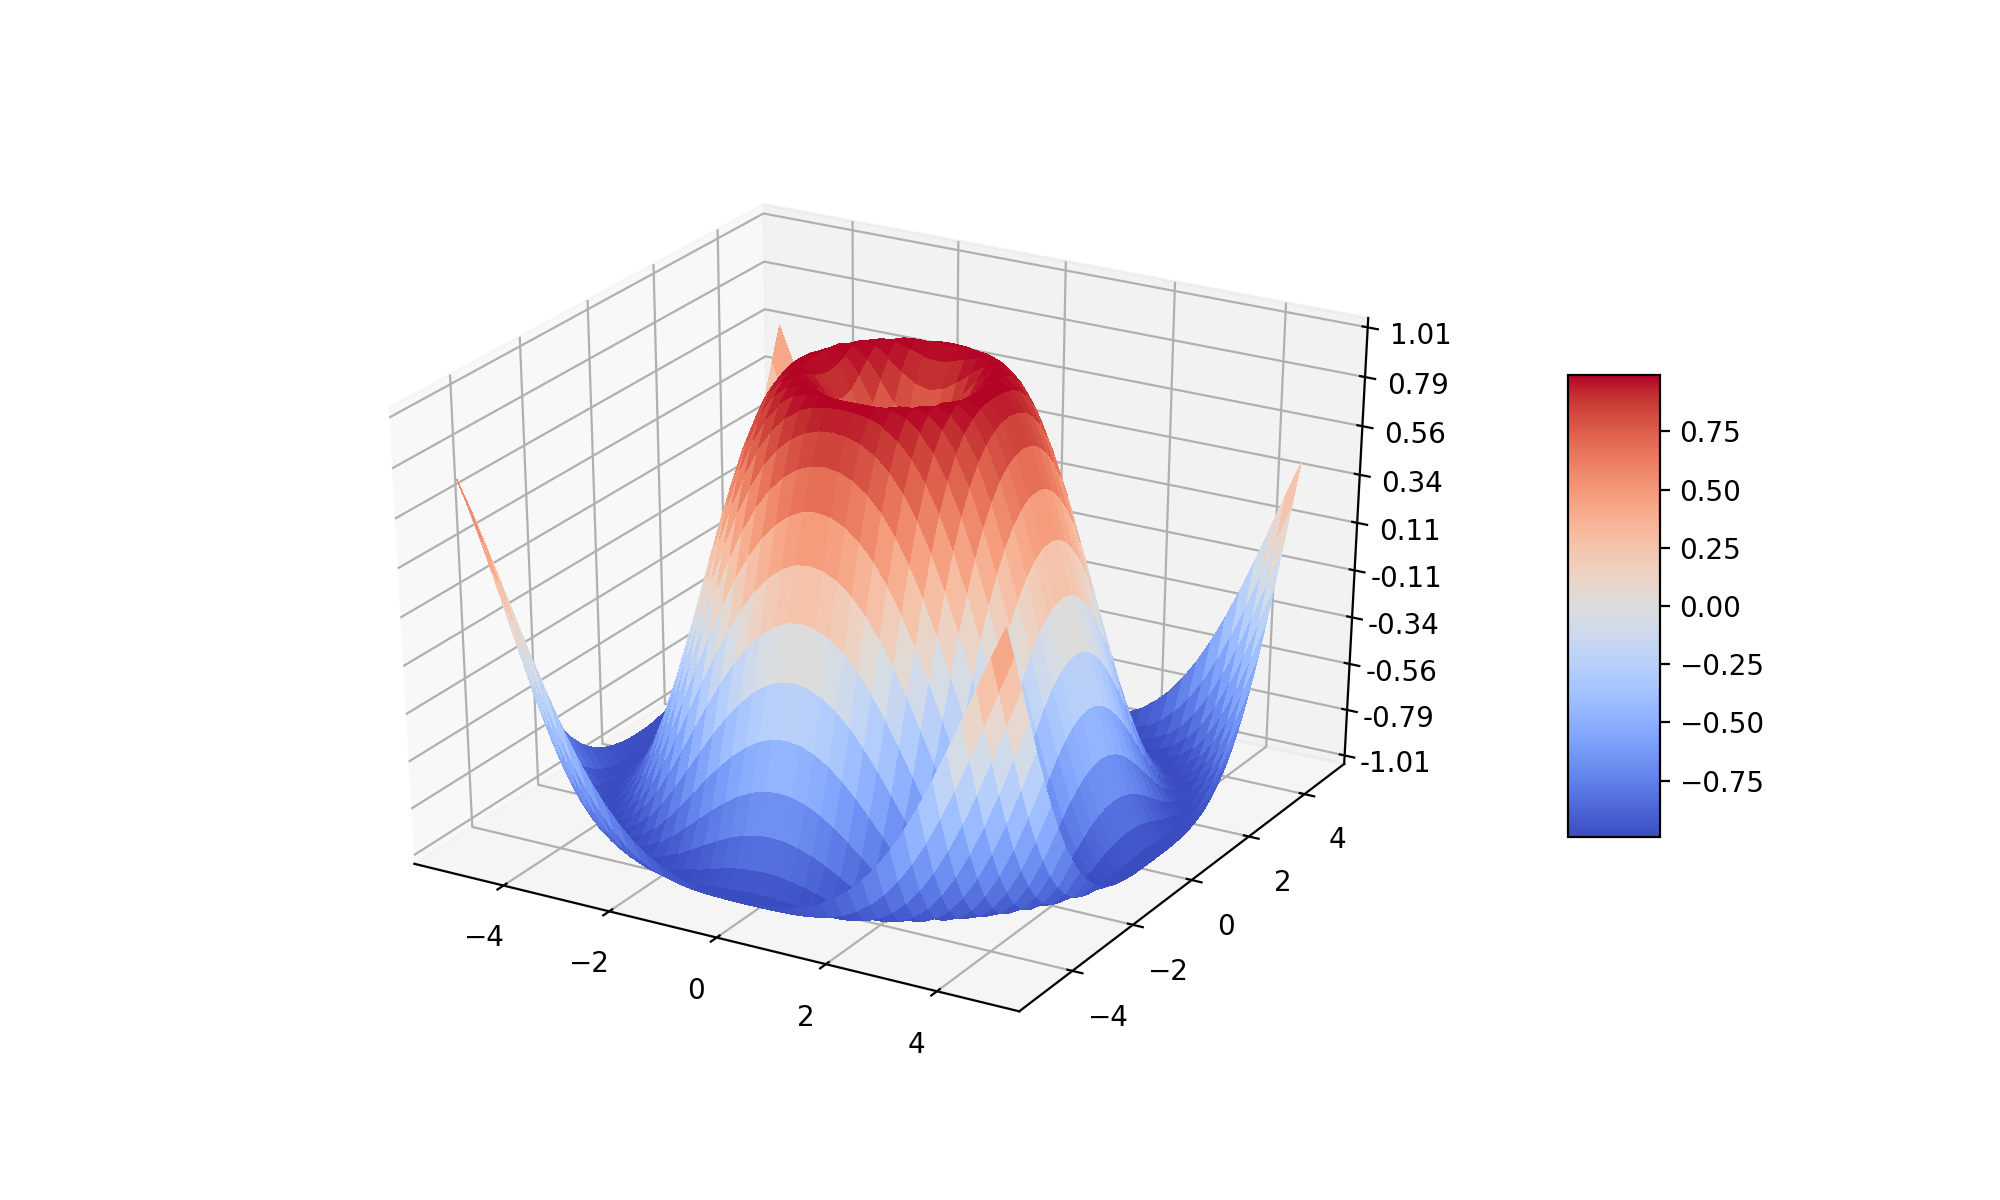
\includegraphics[width=.9\linewidth]{./image/3d_python.png}
\end{center}
\vspace{1mm}
Quelle:
\url{https://matplotlib.org/mpl\_toolkits/mplot3d/tutorial.html} 
\end{block}
\end{column}
\end{columns}
\end{frame}


\begin{frame}[label={sec:orgba2db7a}]{DSP mit Python - Testsystem}
\begin{block}{Hardware}
\begin{itemize}
\item Intel Core i5 3570k, 3000 Mhz
\item 16GB DDR3 1866 MHz, 10-11-10-30 1T
\item Manjaro Linux, Kernel 5.4.44
\end{itemize}
\end{block}

\begin{block}{Software}
\begin{itemize}
\item numpy 1.18.5
\item scipy 1.4.1
\item matplotlib 3.2.1
\item Octave 5.2.0
\item gcc 10.1.0
\end{itemize}
\end{block}
\end{frame}


\begin{frame}[label={sec:org8b5e5af}]{DSP mit Python - Simulation}
\begin{block}{Konzept}
\begin{itemize}
\item Diversity-Technik (Raumdiversität) mit drei Kanälen
\item 20k samples / Waveform
\item Einzelne Kanäle zeitlich versetzt
\end{itemize}
\end{block}

\begin{block}{Durchführung}
\begin{itemize}
\item Umsetzung in Octave, Python, C
\item Rauschminderung via Averaging
\item Upsampling via FFT
\item Delay-Korrektur via cross-correlation
\end{itemize}
\end{block}
\end{frame}


\begin{frame}[label={sec:org6bf0059}]{DSP mit Python - Entwicklung Python}
\begin{itemize}
\item Zuerst Entwicklung des Octave Script
\item Daraus Entwicklung des Python Script 
\begin{itemize}
\item So nah wie möglich mit Octave Script
\end{itemize}
\item Aquivalente Funktionen von den drei Bibliotheken finden:
\begin{itemize}
\item Argumente anpassen 
\begin{itemize}
\item insbesondere Nummerierung von Indizes (Octave 1 bis N; Python 0 bis N-1)
\end{itemize}
\item Rückgabewerte anpassen 
\begin{itemize}
\item (z.B. numpy.arange => ndarray 0 bis N-1; Octave vektor => 1:N)
\end{itemize}
\end{itemize}
\end{itemize}
\end{frame}


\begin{frame}[fragile,label={sec:orgf47ca15}]{DSP mit Python - Codevergleich}
 \begin{block}{Python}
\begin{verbatim}
for i in range(avg_num):
    ch1_waveform_avg += ch1_waveforms[i]

ch1_waveform_avg /= avg_num
\end{verbatim}
\end{block}
\begin{block}{Octave}
\begin{verbatim}
for i = 1:avg_num
    ch1_waveform_avg += ch1_waveforms(i, :);
endfor

ch1_waveform_avg /= avg_num;
\end{verbatim}
\end{block}
\end{frame}


\begin{frame}[fragile,label={sec:org0826dcb}]{DSP mit Python - Codevergleich}
 \begin{block}{Python}
\begin{verbatim}
ch1_S_up = np.concatenate((ch1_S[0:int(wflen/2)], np.zeros(wflen), 
			   ch1_S[int(wflen/2):wflen]))
...
ch1_waveform_upsamp = np.real(scipy.fftpack.ifft(ch1_S_up)) * 2
\end{verbatim}
\end{block}
\begin{block}{Octave}
\begin{verbatim}
ch1_S_up = [ch1_S(1:wflen/2), zeros(1, wflen), ch1_S(wflen/2+1:wflen)];
...
ch1_waveform_upsamp = real(ifft(ch1_S_up)) * 2;
\end{verbatim}
\end{block}
\end{frame}


\begin{frame}[label={sec:org7a17036}]{DSP mit Python - Codevergleich}
\begin{block}{Vorteile Python}
\begin{itemize}
\item Highlevel Programmiersprache -> mehr Flexibilität
\item Mit NumPy und SciPy Libraries -> etwas schneller
\item Vgl. Matlab -> kostenlos "open-source" Software
\begin{itemize}
\item Von einer größeren Community entwickelt
\item Einfacher für Dritte die Code/Ergebnisse zu benutzen
\end{itemize}
\end{itemize}
\end{block}
\begin{block}{Vorteile Octave (Matlab)}
\begin{itemize}
\item Speziell für diesen Art von Anwendung entwickelt
\begin{itemize}
\item Keine zusätzliche Bibliotheken benötigt
\end{itemize}
\item Code ist teilweise einfacher zu verstehen und schreiben
\item In vielen Bereichen bereits etabliert
\begin{itemize}
\item Umstellung zu Python kostet Zeit und Arbeit
\end{itemize}
\end{itemize}
\end{block}
\end{frame}


\begin{frame}[label={sec:org8a102be}]{DSP mit Python - Geschwindigkeit}
\begin{itemize}
\item Teilweise Unterscheide zwischen Python Bibliothekten
\item SciPy-fft war 2 ms schneller als numpy-fft
\end{itemize}
\begin{block}{Computetime verschiedene Codes:}
\begin{itemize}
\item Python: \textasciitilde{}18.3 ms
\item Ocatve: \textasciitilde{}26.3 ms
\item C: \textasciitilde{}99.7 ms
\end{itemize}
\end{block}
\end{frame}


\begin{frame}[label={sec:org5ba8ffc}]{DSP mit Python - Geschwindigkeitsanalyse}
\begin{itemize}
\item Octave / numpy nutzen BLAS / LAPACK
\item Optimiert für Vektor- u. Matrixoperationen
\item Vorteile entsprechend auch bei Scipy
\item Beachtliche Geschwindigkeit bei geringem Entwicklungsaufwand
\end{itemize}
\end{frame}


\begin{frame}[label={sec:org6ab339b}]{DSP mit Python - FPGA}
\begin{block}{NI cRio}
\begin{itemize}
\item Embedded System mit RT Linux und FPGA
\item FPGA kann u.a. via LabWiew programmiert werden
\item FPGA kann via API von Code angesprochen werden
\item Geringer Entwicklungsaufwand
\end{itemize}
\end{block}
\end{frame}


\begin{frame}[fragile,label={sec:org96d236b}]{DSP mit Python - FPGA}
 \begin{block}{Beispiel cRio Python Code}
\begin{verbatim}
with Session("MyBitfile.lvbitx", "RIO0") as session:
    my_control = session.registers['My Control']
    my_indicator = session.registers['My Indicator']
    my_control.write(4)
    data = my_indicator.read()
    print(data)  # prints 16
\end{verbatim}
\end{block}
\begin{block}{Beispiel cRio LabView FPGA}
\hspace{5mm}
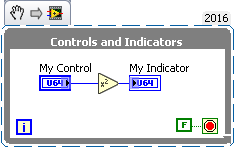
\includegraphics[width = 0.3\textwidth]{image/labview_fpga.png}

\vspace{10mm}
Quelle:
\url{https://nifpga-python.readthedocs.io/en/latest/examples/basic\_examples.html}
\end{block}
\end{frame}


\begin{frame}[label={sec:orgef6bc92}]{DSP mit Python - FPGA}
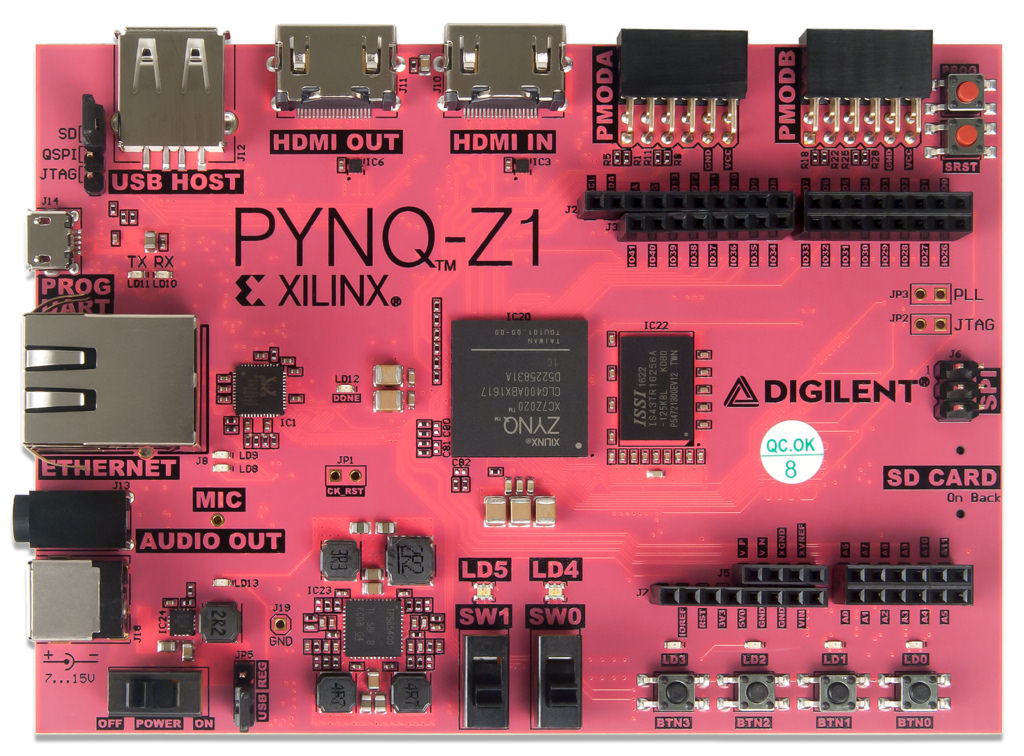
\includegraphics[width = 0.5\textwidth]{image/pynq.jpg}
\begin{block}{Xilinx PYNQ}
\begin{itemize}
\item Entwicklung via Jupyter Notbook im Webbrowser
\item Kostengünstige Boards verfügbar
\item Für privatgebrauch geeignet
\end{itemize}

\vspace{15mm}
Quelle Bild:
\url{https://shop.trenz-electronic.de/media/image/47/bb/33/29034\_1.jpg}
\end{block}
\end{frame}


\begin{frame}[label={sec:org465a824}]{DSP mit Python - Ende}
\begin{block}{ENDE!}
\end{block}
\end{frame}


\begin{frame}[label={sec:org0861488}]{DSP mit Python - Quellen}
\begin{itemize}
\item \url{https://www.scipy.org/}
\item \url{https://numpy.org/}
\item \url{https://matplotlib.org/}
\item \url{https://www.geeksforgeeks.org/python-lists-vs-numpy-arrays/}
\item \url{https://matplotlib.org/mpl\_toolkits/mplot3d/tutorial.html}
\item \url{http://www.pynq.io/}
\item \url{https://nifpga-python.readthedocs.io/en/latest/}
\end{itemize}
\end{frame}
\end{document}
